\documentclass[../report.tex]{subfiles}

\begin{document}
\subsection{Tác tử - Agent}
Một tác tử phần mềm, hay gọi tắt là tác tử là một chương trình máy tính tồn tại trong một môi trường nhất định, 
tự động hành động phản ứng lại sự thay đổi của mội trường nhằm đáp ứng một mục tiêu đã được thiết kế trước. 
Thoả mãn các tính chất sau: 
\begin{itemize}
    \item Bền bỉ - Code không được thực thi theo yêu cầu mà chạy liên tục và tự động quyết định 
        khi nào nên thực hiện hành động nào. 
    \item Tự động - Có khả năng lựa chọn nhiệm vụ, sắp xếp mức độ ưu tiên, hành động hướng mục tiêu, 
        có khả năng tự quyết định mà không cần can thiệp từ con người. 
    \item Xã hội - Có khả năng hợp tác để thực hiện nhiệm vụ thông qua giao tiếp và phối hợp. 
    \item Phản ứng - Tác tử nhận thức từ môi trường và phản ứng lại nó một cách hợp lý. 
\end{itemize}

\subsubsection{Phân biệt tác tử với chương trình}
Tất cả tác tử là chương trình, nhưng chương trình có thể không là tác tử. Sự khác biệt đến từ các tính chất cơ bản của tác tử so với 
một chương trình bất kì. 

\subsubsection{Phân biệt tác tử với đối tượng}
\begin{itemize}
    \item Tác tử có tính tự động hơn là đối tượng.
    \item Tác tử có sự mềm dẻo trong hành vi, có sự phản ứng, tính xã hội. 
    \item Tác tử có thể có nhiều hơn một luồng xử lý. 
\end{itemize}

\subsubsection{Phân biệt tác tử với hệ chuyên gia}
\begin{itemize}
    \item Hệ chuyên gia không được gắn với môi trường. 
    \item Hệ chuyên gia không được thiết kế với khả năng phản xạ. 
    \item Hệ chuyên gia không xét đến tính xã hội của các vấn đề.
\end{itemize}

\subsection{Tác tử thông minh - Intelligent Agent}
Tác tử thông minh là một thực thể tự động, tiếp nhận thông tin từ môi trường và có khả năng tương tác lại môi trường 
và hướng hành động của nó nhằm đạt được một mục tiêu nào đó.
Tác tử thông minh có thể học và sử dụng kiến thức để đạt được mục tiêu. \cite{intelligent-agent-wiki}

\begin{figure}[H]
\centering
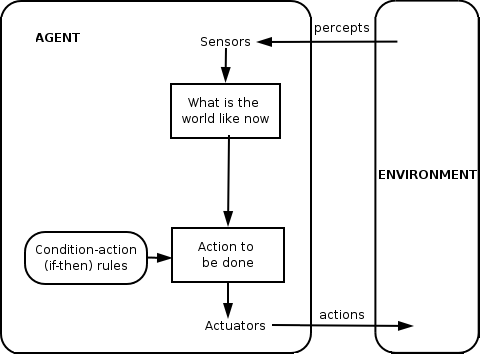
\includegraphics[width=10cm]{figures/simple-reflex-agent.png}
\caption{Simple reflex agent}
\end{figure}

Tác tử thông minh có thể có các đặc trưng sau: 
\begin{itemize}
    \item Có thể bổ sung các quy tắc (rule) giải quyết bài toán. 
    \item Thích ứng với môi trường một cách trực tuyến và thời gian thực. 
    \item Có khả năng phân tích được hành động của bản thân, sự thành công và thất bại. 
    \item Học và cải thiện thông qua tương tác với môi trường. 
    \item Học nhanh chóng từ một lượng dữ liệu lớn. 
    \item Có bộ nhớ để lưu trữ và truy cập. 
    \item Có các tham số để đại diện bộ nhớ ngắn hạn và dài hạn, tuổi tác, mức độ quên, \ldots 
\end{itemize}


\subsection{Hệ đa tác tử - Multi-agent System}
Hệ đa tác tử (multi-agent system) là một hệ tính toán được tạo thành bởi nhiều tác tử thông minh \cite{multi-agent-system-wiki}.
Hệ đa tác tử có thể được sử dụng để giải các bàn toán khó hoặc không thể giải bằng các phương pháp đơn tác tử hoặc một hệ đơn khối nào. 
Hệ đa tác tử được cấu thành bởi các tác tử và môi trường của nó. 

Các tác tử trong hệ đa tác tử có thể chia thành:
\begin{itemize}
    \item Tác tử thụ động hay ``tác tử không có mục đích'' (Ví dụ: vật cản).
    \item Tác tử chủ động với mục đích đơn giản (Ví dụ: xe cộ). 
    \item Tác tử nhận thức với tính toán phức tạp. 
\end{itemize}

Môi trường của các tác tử có thể chia thành:
\begin{itemize}
    \item Ảo.
    \item Rời rạc.
    \item Liên tục. 
\end{itemize}

Môi trường cũng có thể được tổ chức dựa theo các thuộc tính như ``khả năng tiếp cận'', ``tính xác định'', ``tính động'', ``tính rời rạc'',
``tính giai đoạn'', ``số chiều''. 

Đặc trưng của hệ đa tác tử: 
\begin{itemize}
    \item Tự trị: Độc lập ít nhất một phần, tự nhận thức, tự động.
    \item Tầm nhìn giới hạn: Không có tác tử nào có một tầm nhìn cho toàn bộ môi trường, hoặc hệ thống quá phức tạp để
        một tác tử có thể khai thác được lượng kiến thức đó. 
    \item Phân cấp: Không tác tử nào được chỉ định là tác tử chỉ huy. 
\end{itemize}

Hệ đa tác tử đa phần được thực hiện bằng chương trình giả lập. Hệ thống thực hiện lần lượt từng ``bước thời gian''. 


\end{document}
